%!TEX root = uber.tex

\section{Empirical Experiments}

\begin{frame}{Data Sources}
\begin{itemize}
	\item<1->\textcolor{BlueGreen}{\textbf{NYC taxi rides dataset (2015-2016)}}
	\begin{itemize}
		\item[--]<1-> Over 200,000 taxi rides per day, 29 city-zones.
		\item[--]<1-> Pickup/ dropoff times and location co-ordinates.
		\vspace{0.2cm}
		\item[]<2-> \textbf{\alert{Used to generate time-evolving empirical transition matrix ($F$)}}
		\vspace{0.2cm}
	\end{itemize}
	\item<3->\textcolor{BlueGreen}{\textbf{Uber Rides API}}
	\begin{itemize}
		\item[--]<3-> Provides estimates for price and travel time.
		\item[--]<3-> Surge multiplier.
		\vspace{0.2cm}
		\item[]<4-> \textbf{\alert{Used to generate rewards matrix ($R$) and travel time matrix ($T$)}}
		\vspace{0.2cm}
	\end{itemize}
	\item<5->\textcolor{BlueGreen}{\textbf{Methodology:}}
	\only<5>{
		\begin{figure}
		\centering
		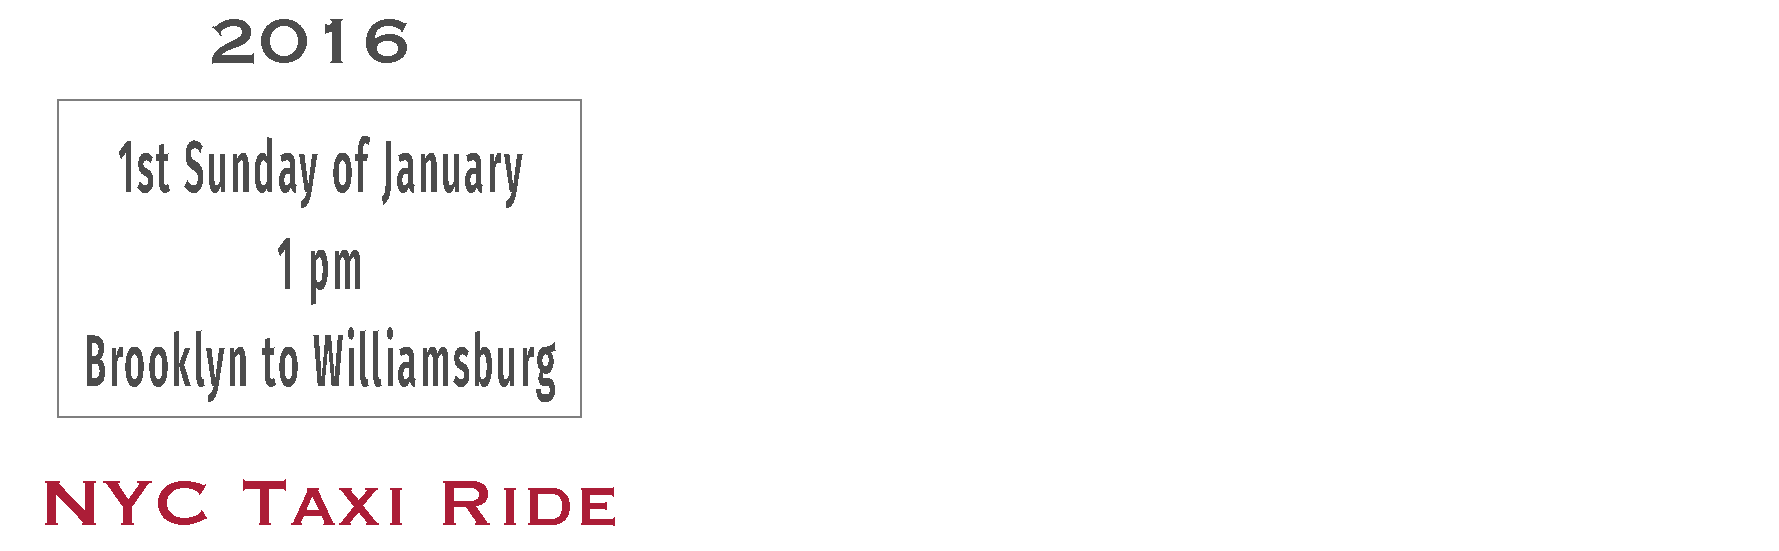
\includegraphics[scale=0.25]{figures/methodology0.pdf}
		\end{figure}
	}
	\only<6>{
		\begin{figure}
		\centering
		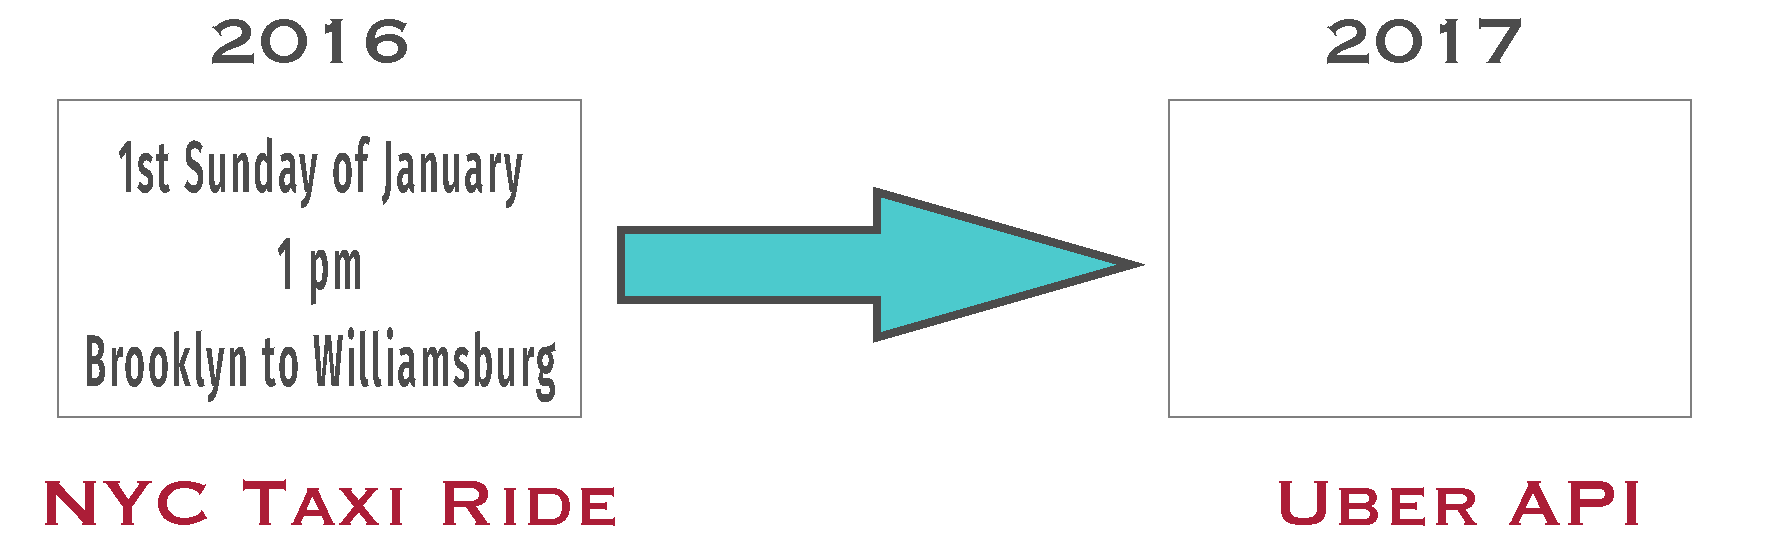
\includegraphics[scale=0.25]{figures/methodology1.pdf}
		\end{figure}
	}
	\only<7>{
		\begin{figure}
		\centering
		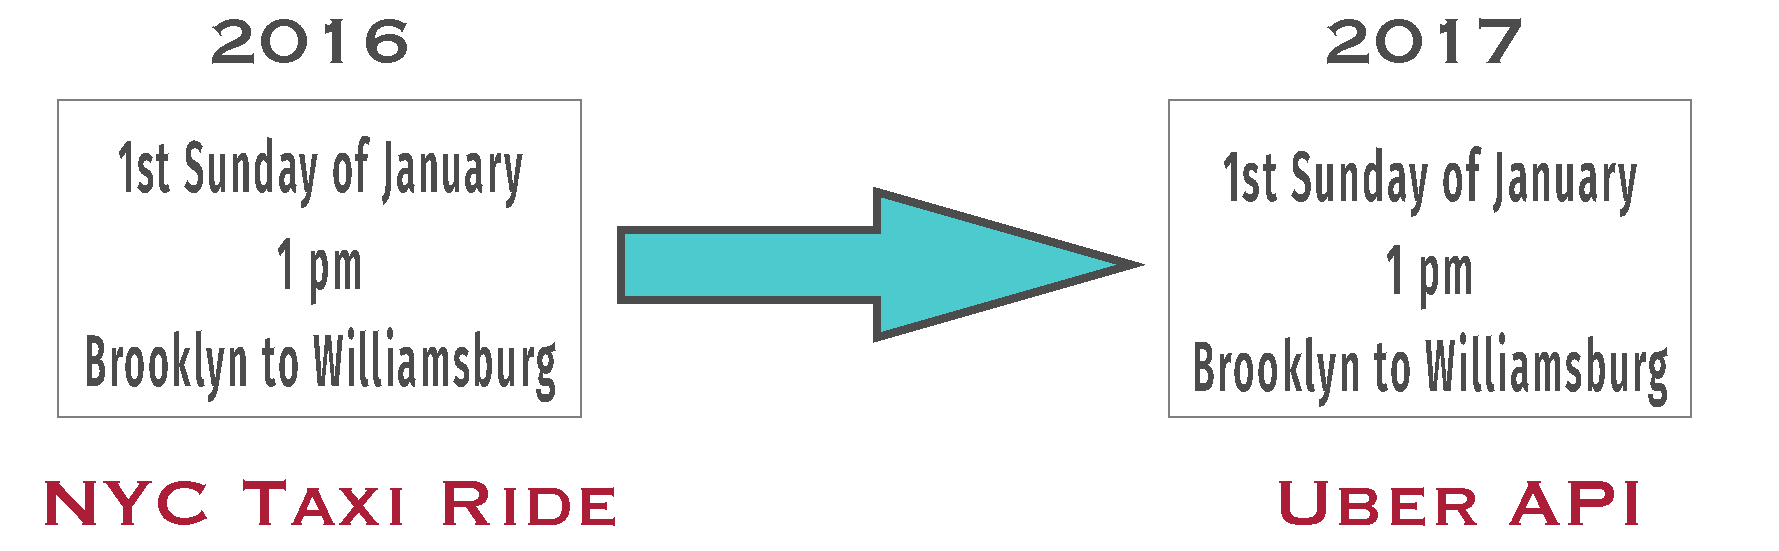
\includegraphics[scale=0.25]{figures/methodology2.pdf}
		\end{figure}
	}
\end{itemize}
\end{frame}

\begin{frame}{Data Processing}
\begin{itemize}
	\item<1-> \textcolor{BlueGreen}{\textbf{Generation of input matrices:}}
	\begin{itemize}
		\item[--] Discretize time into 10 minute steps i.e. \textcolor{BlueGreen}{$N=144$} for a day long strategy.
		\vspace{0.2cm}
		\item[--] For time-evolving matrices \textcolor{BlueGreen}{$F^{(t)}, R^{(t)}$} and \textcolor{BlueGreen}{$T^{(t)}$}, aggregate observations within a 30-minute sliding window centered around time step $t$.
		\vspace{0.2cm}
		\item[--] Use \textcolor{BlueGreen}{passenger arrival} and \textcolor{BlueGreen}{taxi arrival rates} to compute probability of finding a passenger at a particular time.
	\end{itemize}
	\vspace{0.2cm}
	\item<2-> \alert{\textbf{Concerns:}}
	\begin{itemize}
		\item[--] Does NYC taxi data reflect same trends as Uber?\\
		\uncover<3->{\alert{\textcite{chen2015peeking}} have explored this!}
		\item[--] Endogenous relationship of surge.
	\end{itemize}
\end{itemize}
\pause
\uncover<4->{\alert{Better data can be easily incorporated!}}
\end{frame}

% \begin{frame}{Data Collection}
% \textcolor{BlueGreen}{\textbf{Data sources:}}
% \begin{itemize}
% 	\item<1-> \textbf{NYC taxi rides dataset (2015-2016)}
% 	\begin{itemize}
% 		\item[--]<2-> Discretize day into 144 time-steps, each 10 minutes apart.
% 		\item[--]<2-> For time evolving matrix $F$, consider a 30 minute long sliding window centered around each time step $t$.
% 		\item[--]<2-> Use origins and destinations to compute probability of finding a passenger within 10 minutes.
% 	\end{itemize}
% 	\item<1->\textbf{Uber Rides API}
% 	\begin{itemize}
% 		\item[--]<3-> `Re-create' rides from NYC taxi data on exact same day and time but 1 year later by querying Uber API.
% 		\item[--]<3-> Use API response to populate time-evolving matrices $T$ and $R$.
% 		\item[--]<3-> Query surge multiplier every 5 minutes.
% 	\end{itemize}
% \end{itemize}
% \pause
% \uncover<4->{\alert{We do not account for endogenous relationship between demand and surge multiplier.}}
% \end{frame}

\begin{frame}{Performance of Strategies}
\begin{itemize}
	\item 100 simulated drivers for each strategy.
	\begin{itemize}
		\item[--] Random home zone.
		\item[--] 8 hour work-day i.e. $B=48$.
		\item[--] Non-flexible strategy drivers work from 9AM-5PM.
		\item[--] Train policy on data from $\mathrm{week}_i$.
		\item[--] Simulate driver with above policy in $\mathrm{week}_{i+1}$.
	\end{itemize}
\end{itemize}
\pause
\alert{Average 47\% increase in median earnings per day!}
\begin{figure}
	\centering
	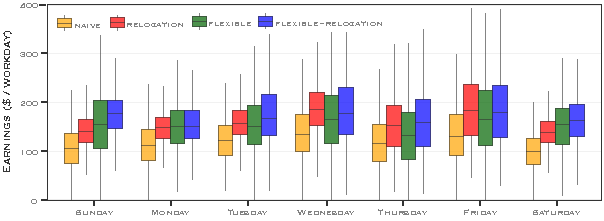
\includegraphics[width=0.85\paperwidth]{figures/daily_simulated_earnings.pdf}
	% \caption{Daily simulated earnings averaged over 10 weeks.}
\end{figure}
\end{frame}

\begin{frame}{Best zones to re-locate to}
\begin{figure}
	\centering
	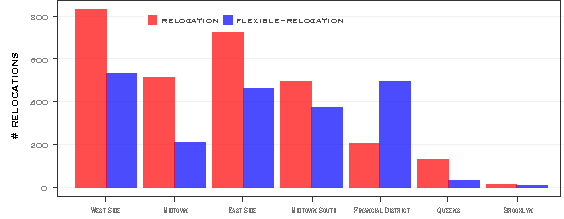
\includegraphics[width=0.85\paperwidth]{figures/relocation_endzones.pdf}
	% \caption{Preferred zones to relocate.}
\end{figure}
\alert{Relocation strategy drivers: exploit spatial variation in Manhattan.}
\end{frame}

\begin{frame}{Best time to drive}
\begin{figure}
	\centering
	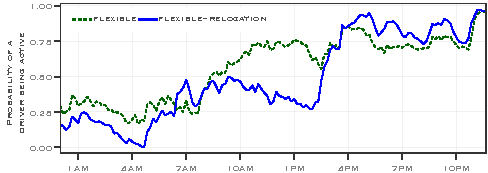
\includegraphics[width=0.85\paperwidth]{figures/simulated_schedules.pdf}
	% \caption{Preferred working schedules.}
\end{figure}
\alert{Flexible-Relocation strategy drivers: exploit the temporal variation in Manhattan.}
\end{frame}

\begin{frame}{To chase surge or not?}
\begin{itemize}
	\item Anecdotally, Uber drivers \textcolor{BlueGreen}{`chase surge'}.
	\pause
	\item \textbf{Simulate surge chasing:} Re-locate to a surging zone if within a 10 minute ride distance
\end{itemize}
\pause
\begin{figure}
	\centering
	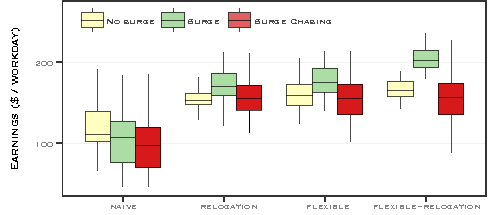
\includegraphics[width=0.65\paperwidth]{figures/simulated_earnings.pdf}
	% \caption{Effect of surge chasing.}
\end{figure}
\alert{Surge Chasing may lead to lower earnings!}
\end{frame}